
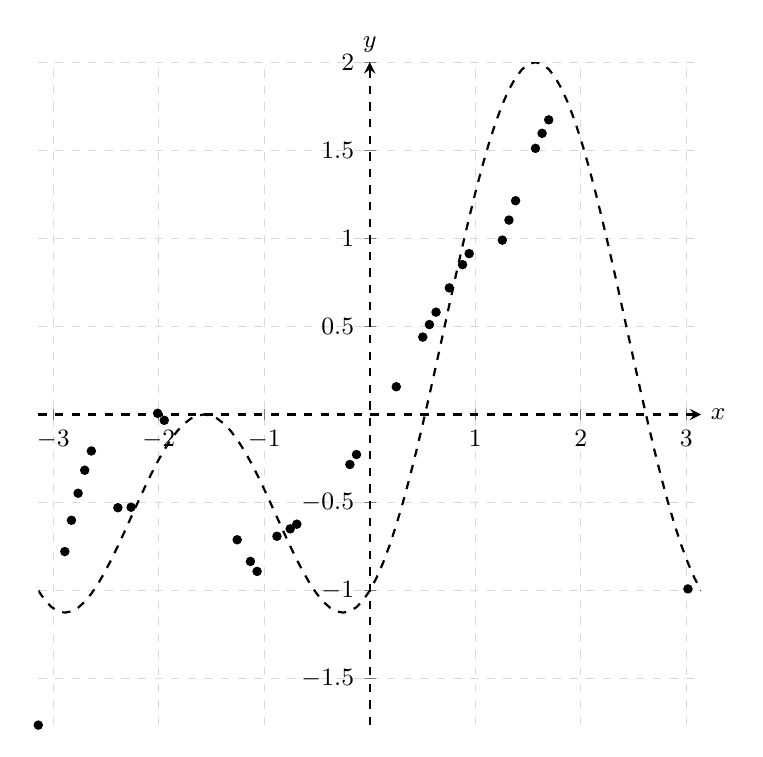
\begin{tikzpicture}
\begin{axis}[
    width=10cm, height=10cm,
    axis lines=middle,
    axis line style={thick, black, dashed},
    xlabel=$x$,
    ylabel=$y$,
    xlabel style={right},
    ylabel style={above},
    grid=major,
    grid style={dashed, gray!30},
    axis background/.style={fill=white},
    tick label style={font=\small},
    label style={font=\small}
]
%% Continuous Function Data
\addplot[no marks, dashed, thick] coordinates {
(-3.14159, -1) (-3.07876, -1.05491) (-3.01593, -1.09392) (-2.9531, -1.11716) (-2.89027, -1.125) (-2.82743, -1.11803) (-2.7646, -1.09709) (-2.70177, -1.0632) (-2.63894, -1.01758) (-2.57611, -0.961606) (-2.51327, -0.896802) (-2.45044, -0.824805) (-2.38761, -0.747338) (-2.32478, -0.666178) (-2.26195, -0.583132) (-2.19911, -0.5) (-2.13628, -0.418549) (-2.07345, -0.34048) (-2.01062, -0.267403) (-1.94779, -0.200808) (-1.88496, -0.14204) (-1.82212, -0.0922765) (-1.75929, -0.0525108) (-1.69646, -0.0235315) (-1.63363, -0.00591203) (-1.5708, 0) (-1.50796, -0.00591203) (-1.44513, -0.0235315) (-1.3823, -0.0525108) (-1.31947, -0.0922765) (-1.25664, -0.14204) (-1.19381, -0.200808) (-1.13097, -0.267403) (-1.06814, -0.34048) (-1.00531, -0.418549) (-0.942478, -0.5) (-0.879646, -0.583132) (-0.816814, -0.666178) (-0.753982, -0.747338) (-0.69115, -0.824805) (-0.628319, -0.896802) (-0.565487, -0.961606) (-0.502655, -1.01758) (-0.439823, -1.0632) (-0.376991, -1.09709) (-0.314159, -1.11803) (-0.251327, -1.125) (-0.188496, -1.11716) (-0.125664, -1.09392) (-0.0628319, -1.05491) (0, -1) (0.0628319, -0.929324) (0.125664, -0.84325) (0.188496, -0.742395) (0.251327, -0.627617) (0.314159, -0.5) (0.376991, -0.360844) (0.439823, -0.211645) (0.502655, -0.0540731) (0.565487, 0.110048) (0.628319, 0.278768) (0.69115, 0.450043) (0.753982, 0.621757) (0.816814, 0.791759) (0.879646, 0.957895) (0.942478, 1.11803) (1.00531, 1.27011) (1.06814, 1.41213) (1.13097, 1.54225) (1.19381, 1.65875) (1.25664, 1.76007) (1.31947, 1.84489) (1.3823, 1.91206) (1.44513, 1.9607) (1.50796, 1.99014) (1.5708, 2) (1.63363, 1.99014) (1.69646, 1.9607) (1.75929, 1.91206) (1.82212, 1.84489) (1.88496, 1.76007) (1.94779, 1.65875) (2.01062, 1.54225) (2.07345, 1.41213) (2.13628, 1.27011) (2.19911, 1.11803) (2.26195, 0.957895) (2.32478, 0.791759) (2.38761, 0.621757) (2.45044, 0.450043) (2.51327, 0.278768) (2.57611, 0.110048) (2.63894, -0.0540731) (2.70177, -0.211645) (2.7646, -0.360844) (2.82743, -0.5) (2.89027, -0.627617) (2.9531, -0.742395) (3.01593, -0.84325) (3.07876, -0.929324) (3.14159, -1) 
};
%% Interpolation Points
\addplot[only marks, mark=*, mark size=1.5pt] coordinates {
(-3.14159, -1.76372) (-2.89027, -0.778422) (-2.82743, -0.600656) (-2.7646, -0.447193) (-2.70177, -0.316538) (-2.63894, -0.207232) (-2.38761, -0.529368) (-2.26195, -0.526388) (-2.01062, 0.00661948) (-1.94779, -0.033026) (-1.25664, -0.711375) (-1.13097, -0.834265) (-1.06814, -0.891058) (-0.879646, -0.691467) (-0.753982, -0.649419) (-0.69115, -0.622854) (-0.188496, -0.284038) (-0.125664, -0.227585) (0.251327, 0.157509) (0.502655, 0.439453) (0.565487, 0.510373) (0.628319, 0.580807) (0.753982, 0.718831) (0.879646, 0.85067) (0.942478, 0.913347) (1.25664, 0.990038) (1.31947, 1.1037) (1.3823, 1.21357) (1.5708, 1.51114) (1.63363, 1.59637) (1.69646, 1.6729) (3.01593, -0.990484) 
};

\end{axis}
\end{tikzpicture}
